\documentclass{article}

\usepackage{graphicx}
\usepackage{amsmath}
\usepackage{amsthm}
\usepackage{amssymb}
\usepackage{url}
\usepackage{multirow}
\usepackage{times}
\usepackage{fullpage}
\usepackage{float}
\usepackage{hyperref}

\linespread{1.25}
\newcommand{\comment}[1]{}

\title{Domain Independent Information Extraction \\
Project Report}
\author{
\begin{tabular}{cc}
	Gowtham Goli & Chakshu Sardana \\
	N17656180 & N10020654 \\	
	\url{sgg308@nyu.edu} & \url{cs4511@nyu.edu}\\
	Dept. of CS & Dept. of CS\\
	\multicolumn{2}{c}{New York University}
\end{tabular}
}
\date{	% replace by ``initial'' or ``final'' as appropriate
1st May, 2016}	% replace by actual date of submission or \today

\begin{document}

\maketitle

\begin{abstract}
Information extraction (IE) is the task of automatically extracting structured information from unstructured and/or semi-structured machine-readable documents available on the web. This paper discusses our implementation of Open Information Extraction from the Web \cite{Banko}, a new extraction paradigm where the system makes a single data-driven pass over its corpus and extracts a large
set of relational tuples without requiring any human input. Our methodology primarily consists of four important modules \textit{Relation Extraction}, \textit{Building Classifier}, \textit{Single Pass Extractor}, \textit{Query Module}. Using Stanford Parser's dependency graph we form tuples. A Naive Bayes classifier is trained to label tuples extracted from a corpus as either trustworthy or untrustworthy. During querying, all similar tuples with a certain overlap are grouped together and ranked. The tuple with the highest rank is returned as the answer to the query.  We then report our experiments on different domain-diverse paragraphs taken from various sources over the web.

\end{abstract}

\section{Introduction}
Information is hidden in vast amount of data that is available now. In Information Extraction, the goal basically is to extract from the documents salient facts about specified types of events, entities or relationships.  Information extraction benefits many text/web applications, for example, integration of product information from various websites, question answering, contact information search, finding the proteins mentioned in a biomedical journal article, and removal of the noisy data \cite{Tang_informationextraction}. Furthermore it can constitute a core component technology in many other NLP applications, such as Machine Translation, Question Answering, Text summarization, Opinion Mining, etc.  Information Extraction is a challenging task; some of the reasons being: use of pronouns like he/she/they etc. make it difficult to analyze, there are many ways of expressing the same fact, and so on. Hence, Information Extraction has traditionally relied on extensive human involvement in the form of hand-crafted extraction rules or hand-tagged training examples and is generally aimed at specific domains like newswire stories, seminar announcements etc. These type of approaches can not work where the number of target relations is very large, or where the target relations cannot be specified in advance. Our approach, which is unsupervised learning based, relies on only unannotated data with no fixed relations which makes it domain independent. This paper discusses our approach to implementing TEXTRUNNER, a fully implemented Open IE system \cite{Banko}, and demonstrates its ability to extract massive amounts of high-quality information from a large Web page corpus, our results and potential future work. Finding semantic relationships between different parts of a sentence is one of the key tasks of Information Extraction. From the corpus, we extract relation tuples of the form \textit{(Subject, Verb, Object)} where Subject and Object are noun phrases. Based on the tuples extracted, queries are answered which is described in detail in the following sections.
 

\section{Approach}
Our approach mainly consists of four important phases

\subsection{Relation Extraction}
In this phase, we parse through the dataset and extract relation tuples from each sentence. Extractions take the form of a tuple $t = (e_i, r_{ij}, e_j)$ where $i < j$ and $e_i$ and $e_j$ are entity strings meant to be the subject and object in the sentence and $r_{ij}$ is a string meant to be the the relationship between them. 
We assumed $e_i$ and $e_j$ to be nouns, $e_i, e_j \in $ \textit{(NNP, NN, NNPS, NNS, CD)} and $r_{ij}$ to be verbs, $r_{ij} \in$  \textit{(VBN, VBP, VB, VBD, VBG, VBZ)}. We used the Jython interace for Stanford Parser \cite{jython} to find all the base nouns and verbs in each sentence. For each noun pairs of the form $(e_i, e_j)$ such that $i<j$, we added all the verbs contained in the sentence thus forming tuples of the form $(e_i, r_{ij}, e_j)$.

Not all of these tuples extracted are guaranteed to hold a valid relationship. So the next step of this phase is to classify the extracted tuples as trustworthy or untrustworthy. To do this, we used the Stanford Parser's dependency graph with collapsed dependencies (the prepositions are added into the relations). The dependency graph for the sentence \textit{Messi has won seven La Liga titles and four UEFA Champions League titles, as well as three Copa del Rey titles.} is shown in Figure \ref{fig:dep}

\begin{figure}[H]
\centering
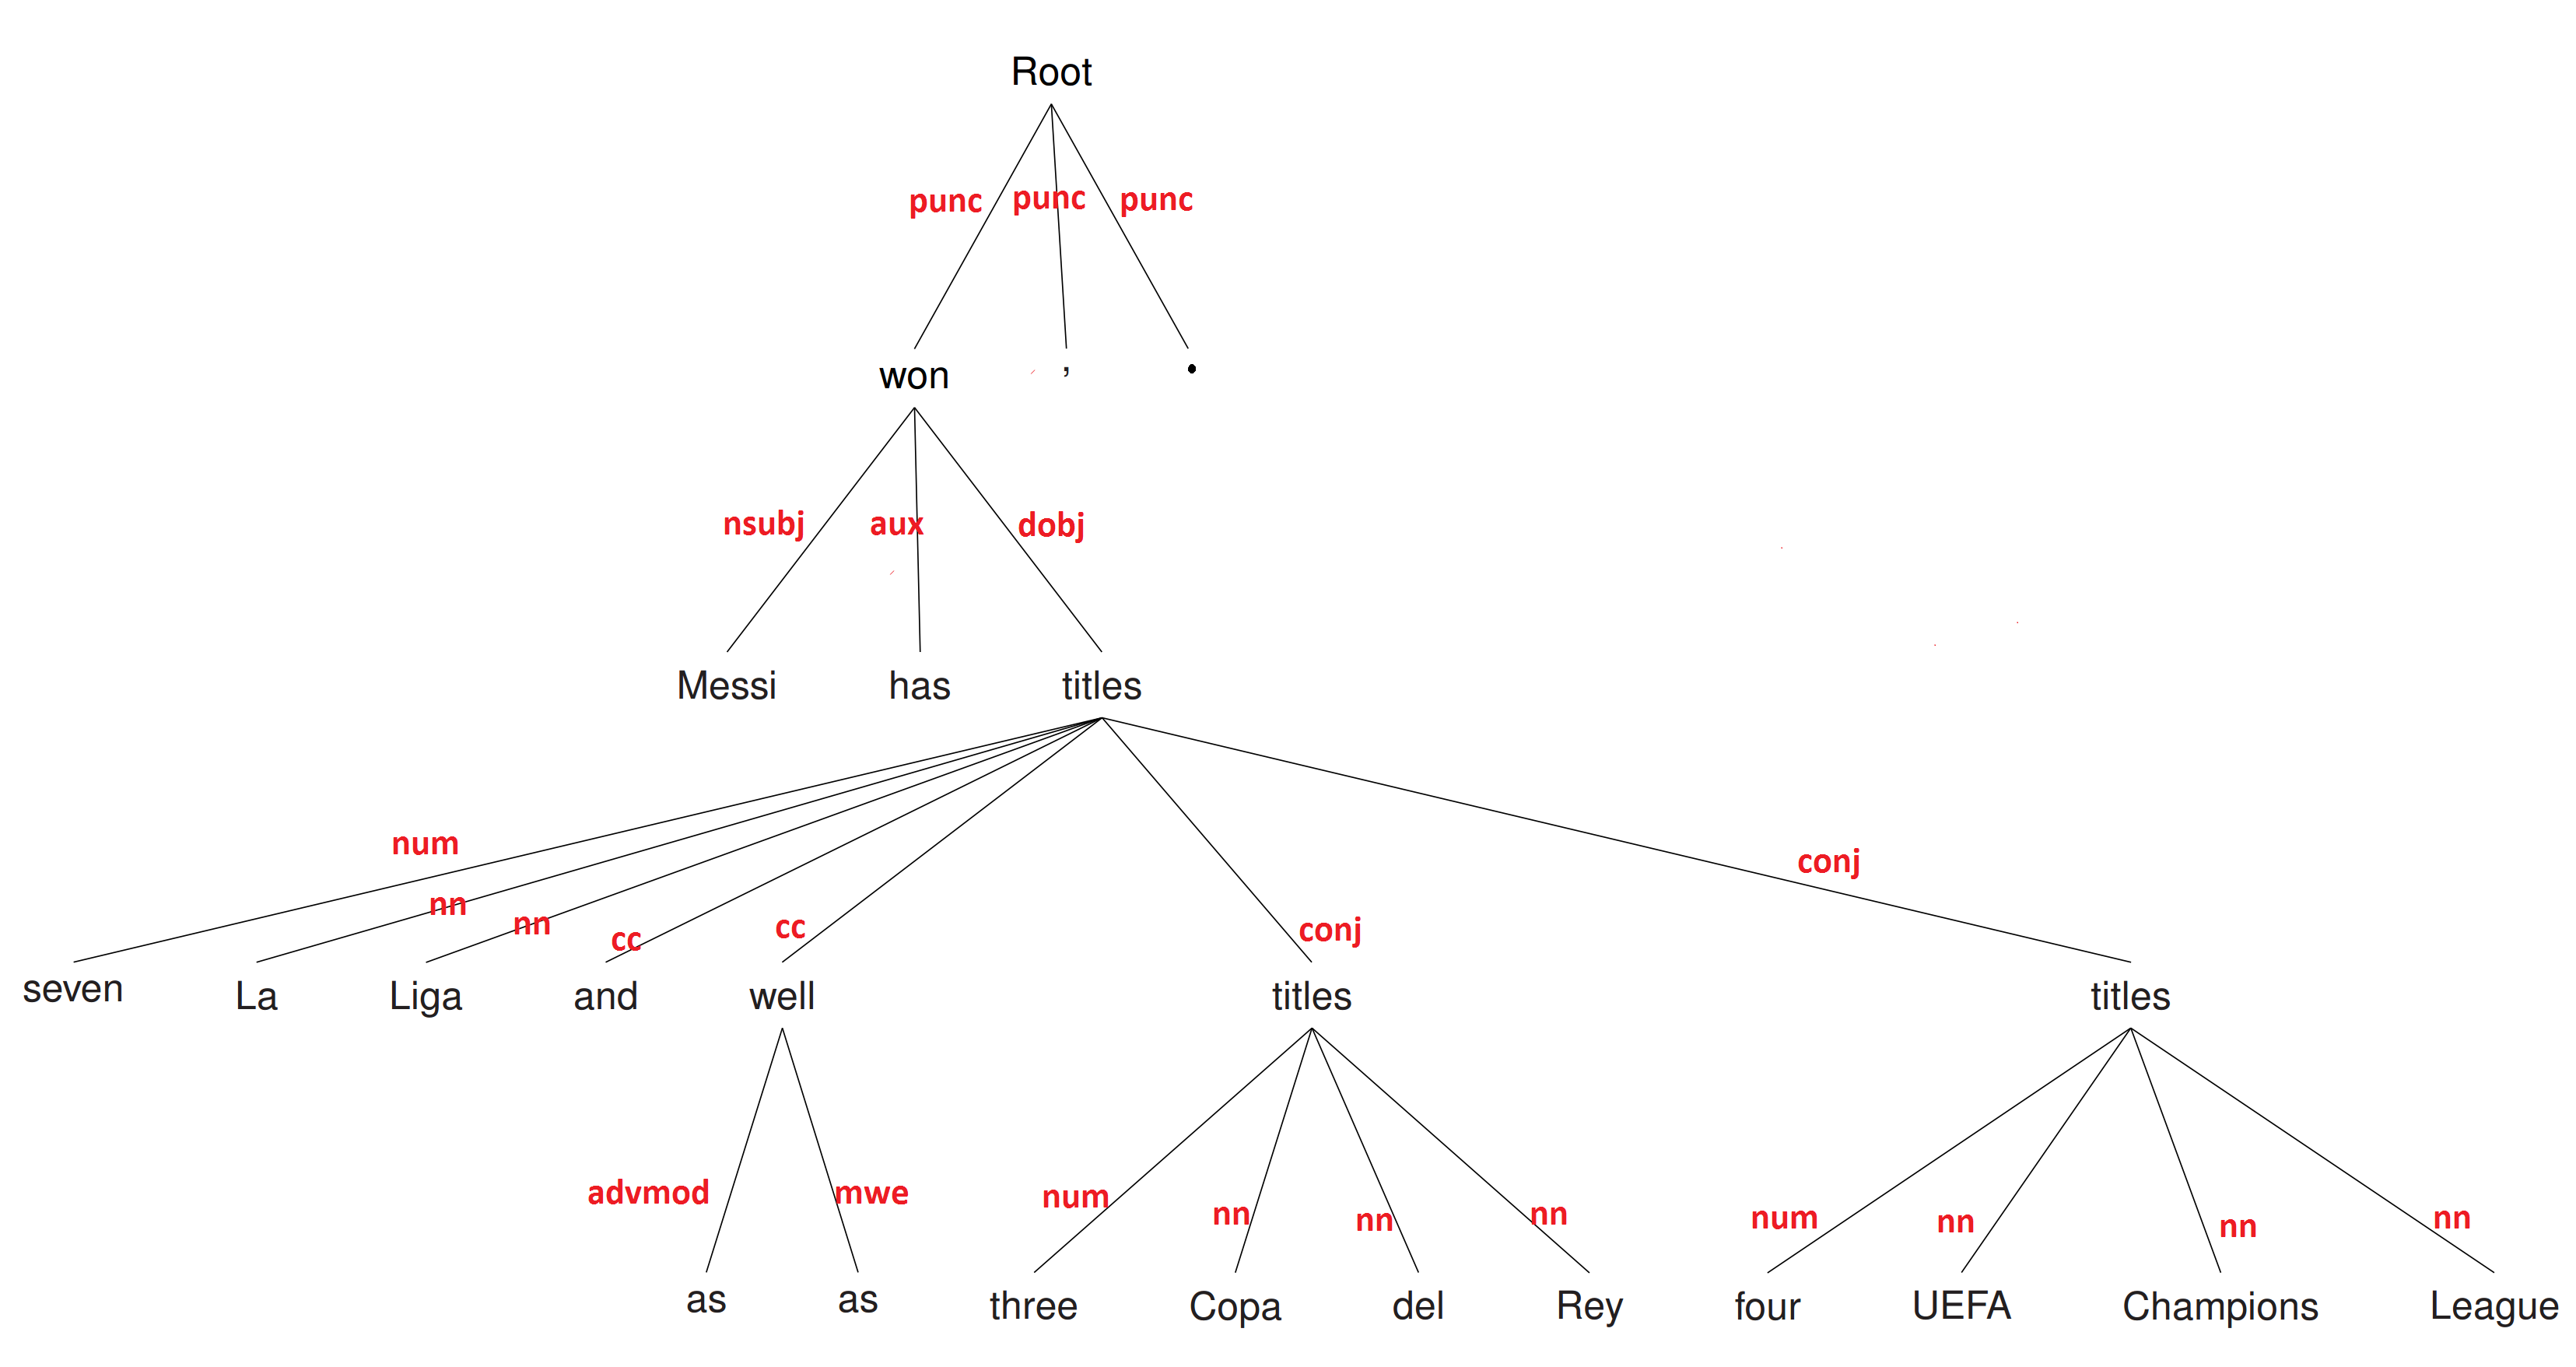
\includegraphics[width=0.9\textwidth]{tree.png}
\caption{Dependency Graph}
\label{fig:dep}
\end{figure}

Using this dependency graph, we classified tuples as trustworthy if they meet certain constraints and untrustworthy otherwise. The following are the constraints we used
\begin{itemize}
\setlength\itemsep{0.05 em}
\item There exists a dependency chain between $e_i$ and $e_j$ that is no longer than a certain threshold value
\item Neither $e_i$ or $e_j$ consists solely of a pronoun.
\end{itemize}

We used Dijkstra's algorithm \cite{Dijkstra} to determine the shortest path between any two nodes in the dependency graph
Few trustworthy and untrustworthy tuples of the above sentence using a threshold value of 2 are shown in the Figure \ref{fig:tuples}

\begin{figure}[h]
\centering
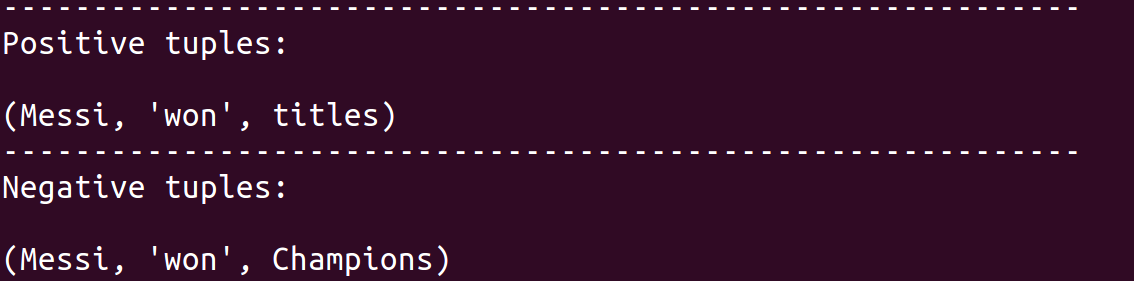
\includegraphics[width=0.8\textwidth]{tuples.png}
\caption{Trustworthy and Untrustworthy tuples}
\label{fig:tuples}
\end{figure}

As it can be observed that there isn't much information being retained in the tuples after extraction, like what titles Messi has won, how many titles he has won etc. To overcome this, we've included the noun phrases instead of just using nouns. Each entity is mapped to the noun phrase it belongs to. If there are multiples noun phrases an entity belongs to, it is mapped to each of the noun phrase. If $e_i$ and $e_j$ belong to the same noun phrase, then they are not mapped. The resulting tuples after this mapping is shown in the Figure \ref{fig:tuples_chunk}. It can be observed that the tuples now contain more information.

\begin{figure}[h]
\centering
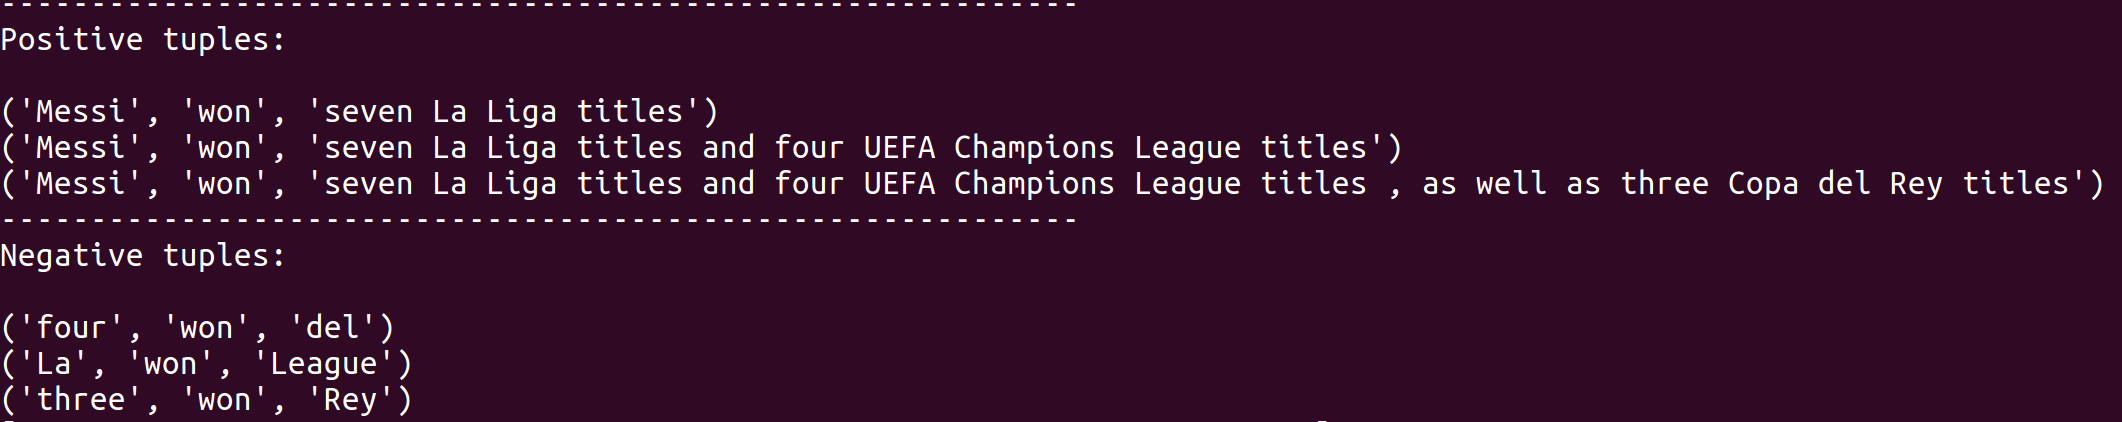
\includegraphics[width=1.0\textwidth]{tuples-chunk.png}
\caption{Trustworthy and Untrustworthy tuples with noun phrases}
\label{fig:tuples_chunk}
\end{figure}

\subsection{Building a classifier}
Using Stanford parser for dependency graphs is computationally expensive and time consuming which is not suitable for real time purposes. To resolve this, we need to build a classifier that will label a given tuple as trustworthy or untrustworthy. For this purpose, every tuple extracted and labeled as either trustworthy or untrustworthy in  \textit{Relation Extraction} is mapped to a feature vector representation, which will be used to build a classifier. All features are domain independent and can be evaluated at the extraction time without the use of a parser. The following are the features included
\begin{itemize}
\setlength\itemsep{0.05 em}
\item Presence of POS tag sequences in the relation $r_{ij}$
\item The number of tokens in $r_{ij}$
\item The number of stopwords in $r_{ij}$
\item Whether or not an object $e$ is found to be a proper noun
\item The part-of-speech tag to the left of $e_i$
\item The part-of-speech tag to the right of $e_j$
\item Distance between $e_i$ and $r_{ij}$ in the sentence
\item Distance between $r_{ij}$ and $e_{j}$ in the sentence
\item Distance between $e_i$ and $r_j$ in the sentence
\end{itemize}

All the above feature vectors obtained for these tuples are then used to train a Naive Bayes classifier.

\subsection{Single Pass extractor}

We perform a single parse over the entire corpus. Using NLTK parse trees \cite{Tree}, we extract noun phrases from each sentence, forming entity tuples of the form $(e_i, e_j)$ where $i < j$. Now all the verbs within the sentence are extracted using their POS tags and are inserted between the entity tuples $(e_i, e_j)$ to form entity-relation tuples $(e_i, r_{ij}, e_j)$. All such entity-relation tuples are extracted from the corpus. These are now sent as input to the Naive Bayes classifier modeled in the above phase. The classifier labels these tuples as either trustworthy or untrustworthy. Only the trustworthy tuples are retained and the untrustworthy ones are discarded. 

\subsection{Query Module}

Due to time constraints, we could only partially implement the \textit{Single Pass extractor} module. For the project to serve as an end to end system, for querying, we retained only the trustworthy tuples and discarded the untrustworthy tuples extracted from the first phase, \textit{Relation Extraction} as suggested by our professor Dr. Grishman. For a given query, all the similar tuples are grouped together and assigned probabilities. The tuple with highest probability is returned as the answer to the query. This is described in detail below. 

The query module accepts 4 types of queries.
\begin{itemize}
\item \_ $q_2$ \_
\item $q_1$ $q_2$ \_
\item $q_1$ \_ $q_3$
\item \_ $q_2$ $q_3$
\end{itemize}
where $q_1$, $q_3$ should be nouns and $q_2$ should be a verb
\subsubsection{\_ $q_2$ \_}

From the trusted tuples, only tuples of the form $(e_i, r_{ij}, e_j)$ where $r_{ij} = q_2$ are retained. Let $n$ be the count of all such tuples. Now from these tuples, similar instances of each entity are grouped together. Any two entities are $e_{i_1}$ and $e_{i_2}$ are considered to be similar if they are either sub string or super string of each other. Let $|e_i|$ be the count of similar instances of $e_i$ and $|e_j|$ be the count of similar instances of $e_j$. Then
\begin{equation*}
P((e_i, r_{ij}, e_j)) = \frac{|e_i| \times |e_j|}{n}
\end{equation*}  

\subsubsection{$q_1$ $q_2$ \_ or $q_1$ \_ $q_3$ or \_ $q_2$ $q_3$}

Consider the case $q_1$ $q_2$ \_. The probabilities in the other two cases can be computed similarly. From the trusted tuples, only tuples of the form $(e_i, r_{ij}, e_j)$ where $e_i = q_1$ and $r_{ij} = q_2$ are retained. Now from these tuples, similar instances of $e_j$ are grouped together. Let $|e_j|$ be it's count. Then
\begin{equation*}
P((e_i, r_{ij}, e_j)) = \frac{|e_j|}{n}
\end{equation*}

The tuple with the maximum probability is returned as the output of the query.

To illustrate using an example, consider the following sentence extracted from our corpus, \textit{The name India is derived from Indus, which originates from the Old Persian word Sindhi.} The \textit{Relation Extraction} module outputs the following trustworthy tuples for this sentence.\\
\textbf{\textit{Trusted tuples:}}\\
\textit{
('The name India', 'derived from', 'Indus , which originates from the Old Persian word Sindhi')\\
('The name India', 'derived from', 'Indus')\\
('Indus', 'originates from', 'Sindhi')\\
('Indus', 'originates from', 'the Old Persian word Sindhi')}

A few example queries that can be formed from the sentence are \textit{(India derived \_\_)} or \textit{(Indus originated \_\_)} or\\ \textit{(\_\_ originated \_\_)} etc. Running the query \textit{(India derived \_\_)} is shown in Figure \ref{fig:query}

\begin{figure}[H]
\centering
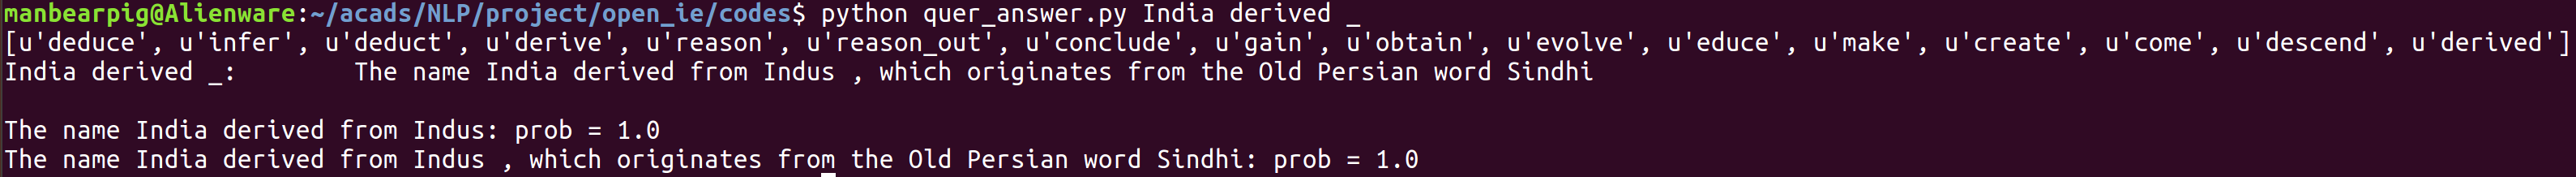
\includegraphics[width=1.1\textwidth]{query.png}
\caption{Answer for Query \textbf{India derived from where?}}
\label{fig:query}
\end{figure}

We used NLTK's Wordnet \cite{Wordnet} to determine synonyms of the tokens in query, which can be seen in the first line of the output (the list of of synonyms for the word \textit{derived} in their stemmed form). Thus, a query of the form \textit{(India deduced \_\_)} would also produce a similar output to the query \textit{(India derived \_\_)} as deduce and derive are both synonyms which is shown in the Figure \ref{fig:query_syno}. The second line contains the answer to the query which is \textit{The name India derived from Indus , which originates from the old Persian word Sindhi} which is followed by all the possible answers to the query with their respective probabilities in decreasing order. In case, an answer couldn't be found, NULL is returned. If two answers have equal probabilities, we considered the answer that contains a bigger noun phrase, thus ensuring more information. For example, in the above sentence the probability for both the answers is equal which is 1.0. However, the later sentence is returned as it carries more information. 

\begin{figure}[H]
\centering
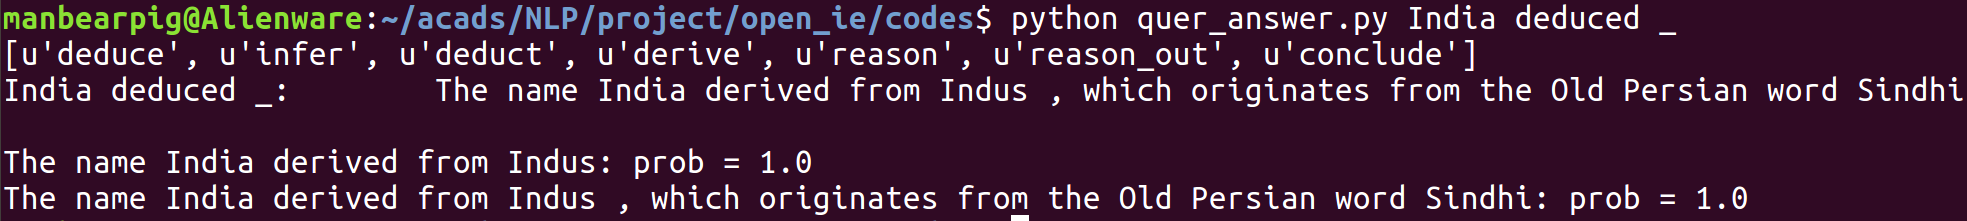
\includegraphics[width=1.0\textwidth]{query_syno.png}
\caption{Answer for Query \textbf{India deduced from where?}}
\label{fig:query_syno}
\end{figure}

\section{Results}
We've analyzed our experimental results by extensive human involvement which was quite tedious. To do this, we extracted a few paragraphs from various sources over the web covering a wide range of domains such as Science, News, Business, Biographies, Sports, Travel etc.

From each of these paragraphs, tuples are formed using \textit{Relation extraction} module, discarding the untrustworthy ones. However, not all the trusted tuples extracted were relevant. For example, some of the tuples lacked context and information, some of them were meaningless etc. A few such examples are shown below classified as Useful and Non-Useful trustworthy tuples.\\
\textbf{Useful trustworthy tuples:}\\
\textit{
('The disappointing performance', 'marked', 'the third straight year in which US GDP figures have missed the estimates made by forecasters')\\
('infections that invade the whole body', 'disable', 'the immune system')\\
('scientists', 'develop', "vaccines that restore immunity in people with systemic or ` whole body ' infections")\\
('The US economy', 'slowed to', 'its weakest pace in two years')\\
('Non-housing investment', 'dropped', '5.9 pc , its largest fall since the second quarter of 2009')\\
('the findings', 'show', 'the capacity of the dendritic cells to display the antigens of new viruses')\\
("Rummenigge 's left", 'sat', 'Pep Guardiola')\\
('the new Dubai tower', 'feature', 'a slender , streamlined structure')
\\
('Lead researcher Dr Jose Villadangos , an immunologist from the Walter and Eliza Institute of Medical Research in Melbourne ,', 'says', 'systemic infections such as malaria or sepsis , a bacterial infection of the blood , overstimulate dendritic cells')
}\\
\textbf{Non-Useful trustworthy tuples:}\\
('Tesla', 'lived in', 'a series of New York hotels')\\
('Tesla', 'lived through', 'his retirement')\\
('The economy', 'grew by', 'just 0.1 pc')\\
('The economy', 'grew in', 'the first quarter of the year')\\
('the post-match banquet in Madrid on Wednesday', 'Karl-Heinz', 'night')\\

As it can be observed, the Useful tuples contained both context and information.

However, the Non-Useful tuples lacked either context or information. For example, \textit{('Tesla', 'lived in', 'a series of New York hotels')} or \textit{('The economy', 'grew by', 'just 0.1 pc')} don't provide any information about when Tesla lived in a series of New York hotels and when the economy grew by 0.1\%. One way to resolve this could be by merging two or more Non-useful tuples so context and information can be improved. For example, \textit{('Tesla', 'lived in', 'a series of New York hotels')} and \textit{('Tesla', 'lived through', 'his retirement')} can be merged to form \textit{('Tesla', 'lived in', 'a series of New York hotels though his retirement')} resulting in a Useful tuple. Similarly, \textit{('The economy', 'grew by', 'just 0.1 pc')} and \textit{('The economy', 'grew in', 'the first quarter of the year')} can be merged to form \textit{('The economy', 'grew by', 'just 0.1 pc in the first quarter of the year')}. Some of the trustworthy tuples were completely worthless due to wrong POS tagging. For example, \textit{('the post-match banquet in Madrid on Wednesday', 'Karl-Heinz', 'night')} doesn't make any sense as \textit{Kar-Heinz} is incorrectly tagged as a verb.


Once the tuples are extracted, all possible queries of the form described in \textit{Query Module} were manually constructed from each paragraph. This amounted to $646$ queries. Each of these queries is then sent to the Query module as an input. Each answer returned by the Query module was checked against the corpus manually to check for it's validity. 433 out of 646 queries were correctly answered resulting in an accuracy of 67\%, (using threshold value of 2, in the dependency graph) . An example of running query \textit(\_\_ detect \_\_) is shown in the figure \ref{fig:query-ex}

\begin{figure}[h]
\centering
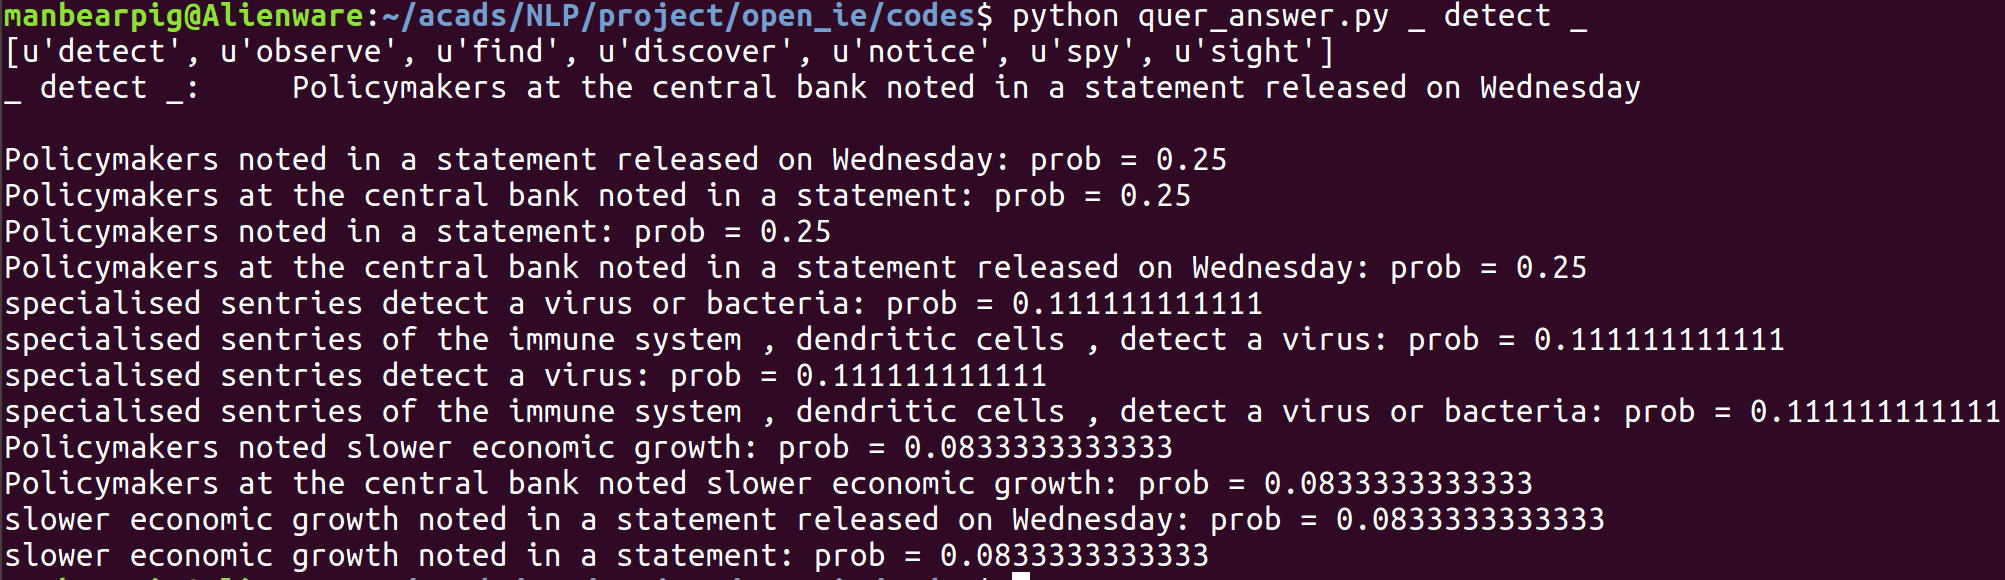
\includegraphics[width=1.0\textwidth]{query_ex.png}
\caption{Answer for Query \textbf{What detects what?}}
\label{fig:query-ex}
\end{figure}

As seen in the figure, the highest ranked answer returned is \textit{Policymakers at the central bank noted in a statement released on Wednesday} (since \textit{notice} and \textit{detect} are synonyms) with a probability of 0.25. In our evaluation, we've marked all such answers as correct. Some of the lesser probable answers returned  are a) \textit{specialised sentries of the immune system , dendritic cells , detect a virus or bacteria} b) \textit{Policymakers at the central bank noted slower economic growth} c) \textit{slower economic growth noted in a statement released on Wednesday}.

\section{Future Work}

In future, we plan to implement capturing context and information from Non-Useful tuples as described above. It is also possible to make logical references using two or more tuples. For example, \textit{('mice', 'injected with', 'a live vaccine')} + \textit{('a live vaccine', 'made of', 'dendritic cells')} + \textit{('dendritic cells', 'exposed to', 'a secondary virus in the laboratory')} $\implies$ \textit{mice injected with a live vaccine made of dendritic cells exposed to a secondary virus in a laboratory}.

Our current corpus is relatively small which isn't good enough to train a robust classifier. We plan to add more training data including corpus from various other domains in addition to our current corpus and include additional features for the classifier. As we have only partially implemented the \textit{Single Pass Extractor}, we plan to integrate this module into the current pipeline so that we can extend our project into a fully functional end to end query answering system. 

\section{Acknowledgements}
We would like to thank our supervisor, Prof. Ralph Grishman, for the patient guidance and advice he has provided throughout the project.

\bibliography{references}{}
\bibliographystyle{plain}
\nocite{*}

\end{document}

